% !TEX root = handbook-physics.tex
%!TEX TS-program = pdflatex
%!TEX encoding = UTF-8 Unicode

\chapter{Motion in non-inertial Frames of Reference}
\label{ch-07}
\zhtitle{非惯性参考系中的运动}

\section{Kinematics of Relative Motion}
\label{sec-7.1}
\zhtitle{相对运动学}
\subsection{}\label{7.1.1} It is assumed in classical (Newtonian) mechanics that distances and time intervals remain unchanged in going over from one frame of reference to any other frame that is in motion in even the most arbitrary manner with re­spect to the first frame. For example, assume that $K$ is 
an inertial frame with origin at point $O^{*}$ and $S$ is a \emph{non-inertial} frame with its origin at point $O$ (\figr{fig-07-01}).
\zhpar{经典（牛顿）力学认为，当参考系变换到另一个以任意方式相对于原参考系运动的参考系时，距离和时间间隔保持不变。例如，设 $K$ 为原点位于点 $O^{*}$ 的惯性参考系，$S$ 为原点位于点 $O$ 的\emph{非惯性}参考系（见\figr{fig-07-01}）。}
\begin{marginfigure}%[!ht]
%\begin{wrapfigure}{r}{0.5\linewidth}
\centering
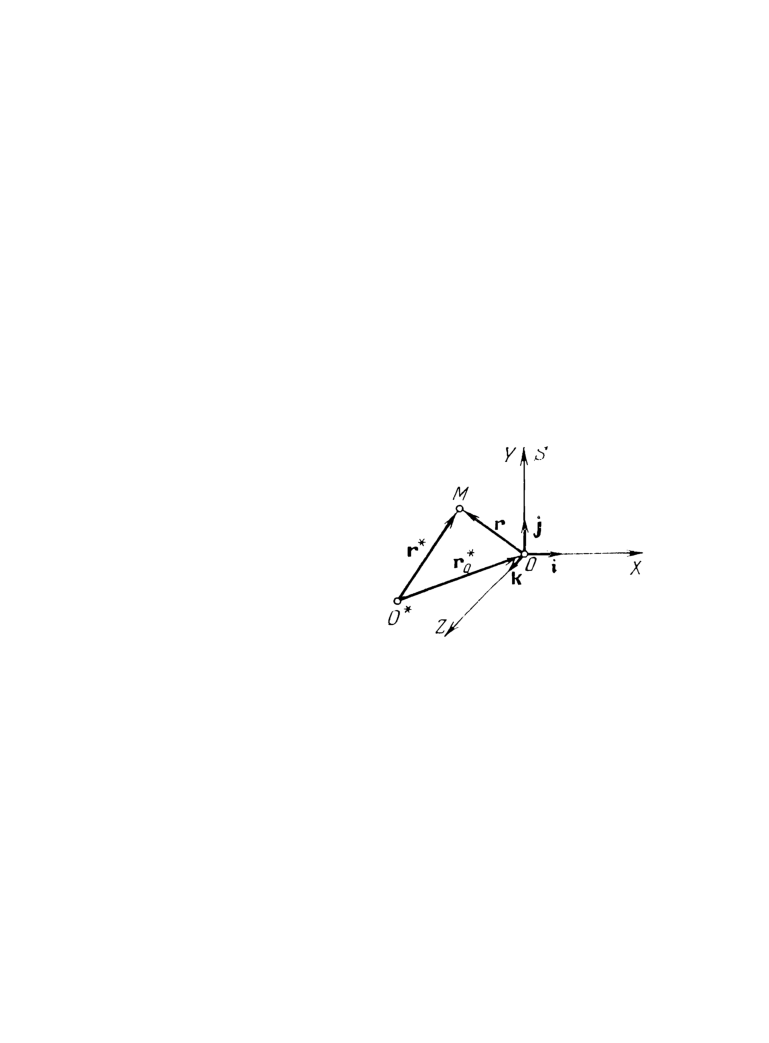
\includegraphics[width=0.8\textwidth]{figs/ch-07/fig-07-01.pdf}
%\input{figs/ch-03/fig-03-01}
%  \vspace{-13pt}
\sidecaption{Inertial and non-inertial frames of reference.\zhcap{惯性参考系与非惯性参考系。}
\label{fig-07-01}}
\end{marginfigure}

In the general case, the mo­tion of frame $S$ with respect to frame $K$ can be regarded as the sum of two motions: translational motion of point $O$ at the velocity $\vb{v}_{0}$ and rotation about this point at the angular velocity $\pmb{\Omega}$. Radius vectors $\vb{r}^{*}$ and $\vb{r}$ of arbitrary particle $M$, measured in frames $K$ and $S$, are related by the equation
\zhpar{一般情况下，参考系 $S$ 相对于参考系 $K$ 的运动可视为两种运动的合成：点 $O$ 以速度 $\vb{v}_{0}$ 作平动，同时绕该点以角速度 $\pmb{\Omega}$ 转动。任意质点 $M$ 在参考系 $K$ 与 $S$ 中测得的位矢 $\vb{r}^{*}$ 与 $\vb{r}$ 之间的关系如下式所示：}
\begin{equation*}%
\vb{r}^{*} = \vb{r}^{*}_{0} + \vb{r},
\end{equation*}
where $\vb{r}^{*}_{0}$ is the radius vector of point $O$ measured in frame of reference $K$.
\zhpar{式中，$\vb{r}^{*}_{0}$ 为在参考系 $K$ 中测得的点 $O$ 的位矢。}

\subsection{}\label{7.1.2} The motion of particle $M$ with respect to any inertial frame of reference $K$, conditionally assumed to be fixed, is called the \emph{absolute motion} of particle $M$. The motion of the same particle with respect to the non-inertial frame of refer­ence $S$ is said to be \emph{relative motion}.
\zhpar{质点 $M$ 相对于任一假定为静止的惯性参考系 $K$ 的运动，称为质点 $M$ 的\emph{绝对运动}。同一质点相对于非惯性参考系 $S$ 的运动，则称为\emph{相对运动}。}

The \emph{relative velocity} $\vb{v}_{r}$ of particle $M$, i.e. its velocity with respect to frame $S$, equals
\zhpar{质点 $M$ 的\emph{相对速度} $\vb{v}_{r}$（即其相对于参考系 $S$ 的速度）如下式所示：}
\begin{equation*}%
\vb{v}_{r} = \dv{x}{t} \vu{i} +\dv{y}{t} \vu{j} + \dv{z}{t} \vu{k}, 
\end{equation*}
where $x$, $y$ and $z$ are the Cartesian coordinates of particle $M$, and $\vu{i}$, $\vu{k}$ and $\vu{k}$ are the unit vectors of the coordinate axes in frame $S$.
\zhpar{式中 $x$、$y$ 和 $z$ 为质点 $M$ 的笛卡儿坐标，$\vu{i}$、$\vu{k}$ 和 $\vu{k}$ 为参考系 $S$ 中坐标轴的单位矢量。}

The \emph{absolute velocity} of particle $M$, i.e. its velocity $\vb{v}$ in the frame of reference $K$, equals
\zhpar{质点 $M$ 在参考系 $K$ 中的速度，即其\emph{绝对速度} $\vb{v}$，如下式所示：}
\begin{equation*}%
\vb{v} = \dv{\vb{r}^{*}}{t}= \vb{v}_{0} + x\dv{\vu{i}}{t}  + y\dv{\vu{j}}{t}  + z \dv{ \vu{k}}{t} + \vb{v}_{r},
\end{equation*}
where $\vb{v}_{0}= \dv*{\vb{r}^{*}_{0}}{t}$ is the absolute velocity of point $O$. Since the unit vectors of moving frame $S$ can change in frame of reference $K$ only due to the rotation of frame $S$ about point $O$ at the angular velocity $\pmb{\Omega}$,
\zhpar{式中 $\vb{v}_{0}= \dv*{\vb{r}^{*}_{0}}{t}$ 为点 $O$ 的绝对速度。由于动参考系 $S$ 的单位矢量在参考系 $K$ 中的变化，只能由该系绕点 $O$ 以角速度 $\pmb{\Omega}$ 转动引起，因此有下列关系：}
\begin{align*}%
\dv{\vb{i}}{t} & = \qty[\pmb{\Omega} \vb{i}], \quad \dv{\vb{j}}{t} = \qty[\pmb{\Omega} \vb{j}], \quad \dv{\vb{k}}{t} = \qty[\pmb{\Omega} \vb{k}] \\
\intertext{and}
\vb{v} & =  \vb{v}_{t} + \vb{v}_{r},
\end{align*}
where $\vb{v}_{t} = \vb{v}_{0}+ \qty[\pmb{\Omega} \vb{k}]$ is the \emph{velocity of transportation} of par­ticle $M$. It is also called the \emph{bulk}, or \emph{drift}, \emph{velocity} and is equal to the absolute velocity of the point of moving frame of ref­erence $S$ (i.e. rigidly fixed in this frame) in which particle $M$ is located at the given instant of time.
\zhpar{式中 $\vb{v}_{t} = \vb{v}_{0}+ \qty[\pmb{\Omega} \vb{k}]$ 为质点 $M$ 的\emph{牵连速度}。它也称为\emph{整体速度}，或称\emph{漂移速度}，等于动参考系 $S$ 中质点 $M$ 在给定时刻所处位置的点（该点相对于此参考系固定）的绝对速度。}

\subsection{}\label{7.1.3} The \emph{relative acceleration} $\vb{a}_{r}$ of particle $M$ (its acceleration with respect to frame $S$) equals
\zhpar{质点 $M$ 的\emph{相对加速度} $\vb{a}_{r}$（即其相对于参考系 $S$ 的加速度）如下式所示：}
\begin{equation*}%
\vb{a}_{r} = \dv[2]{x}{t} \vb{i} +\dv[2]{y}{t} \vb{j} + \dv[2]{z}{t} \vb{k}.
\end{equation*}
The \emph{absolute acceleration} of particle $M$, i.e. its acceleration with respect to frame $K$, equals
\zhpar{质点 $M$ 的\emph{绝对加速度}（即其相对于参考系 $K$ 的加速度）如下式所示：}
\begin{equation*}%
\vb{a} = \dv{\vb{v}}{t} = \vb{a}_{t} + \vb{a}_{C}  + \vb{a}_{r}.
\end{equation*}
Here
\zhpar{其中}
\begin{equation*}%
\vb{a}_{t} = \dv{\vb{v}_{0}}{t} + \left[ \dv{\pmb{\Omega}}{t} \vb{r} \right] + \qty[\pmb{\Omega}[\pmb{\Omega}\vb{r}]],
\end{equation*}
is the \emph{acceleration of transportation} of particle $M$. It is equal to the absolute acceleration of the point in moving frame $S$ in which particle $M$ is located at the given instant of time, and
\zhpar{为质点 $M$ 的\emph{牵连加速度}，它等于质点 $M$ 在给定时刻所处位置处、动参考系 $S$ 中该点的绝对加速度，以及}
\begin{equation*}%
\vb{a}_{C} = 2\qty[\pmb{\Omega}\vb{v}_{r}],
\end{equation*}
is the \emph{Coriolis acceleration} of particle $M$. The Coriolis accelera­tion has its maximum value if the relative velocity $\vb{v}_{r}$ of the particle is perpendicular to the vector $\pmb{\Omega}$ of angular velocity of the moving frame of reference. It is equal to zero if the angle between vectors $\vb{v}_{r}$ and $\pmb{\Omega}$ equals zero or $\pi$, or if even one of these vectors equals zero.
\zhpar{为质点 $M$ 的\emph{科里奥利加速度}。当质点的相对速度 $\vb{v}_{r}$ 与动参考系的角速度矢量 $\pmb{\Omega}$ 相互垂直时，科里奥利加速度达到最大值。当矢量 $\vb{v}_{r}$ 与 $\pmb{\Omega}$ 之间的夹角为零或 $\pi$，或两矢量中至少有一个为零时，科里奥利加速度等于零。}

\section{Inertial Forces}
\label{sec-7.2}
\zhtitle{惯性力}

\subsection{}\label{7.2.1} Newton's laws of motion are not valid in non-inertial frames of reference. In particular, a particle can change the slate of its motion with respect to non-inertial frame S without any action being exerted on the particle by other bodies. A ball, for instance, suspended by a string from the ceiling of a railway coach of a train travelling at uniform velocity in a straight line, deviates backward when the motion of the train is accel­erated and frontward when the motion is decelerated, i.e. it begins to move with respect to a non-inertial frame of reference attached to the coach. But no horizontal forces act on the ball when it deviates.
\zhpar{牛顿运动定律在非惯性参考系中不成立。特别地，质点可以在没有其他物体对其施加作用的情况下，相对于非惯性参考系 $S$ 改变其运动状态。例如，一只用细绳悬挂在天花板上的小球，悬挂于沿直线匀速行驶的列车车厢中。当列车加速时，小球向后偏离；当列车减速时，小球向前偏离。也就是说，小球开始相对于固连在车厢上的非惯性参考系运动，但在此偏离过程中，小球上并不存在任何水平方向的作用力。}

\subsection{}\label{7.2.2} The fundamental law of dynamics for a particle in non-inertial frames of reference can be derived from Newton's second law and the relation between the absolute and relative accel­erations of a particle. It follows from \ssect{7.1.3} that the product of the mass $m$ of a particle by its relative acceleration equals
\zhpar{非惯性参考系中质点的动力学基本定律，可由牛顿第二定律以及质点绝对加速度与相对加速度之间的关系导出。由 \ssect{7.1.3} 可知，质点的质量 $m$ 与其相对加速度的乘积如下式所示：}
\begin{equation*}%
m \vb{a}_{r} = m \vb{a} - m \vb{a}_{t} - m \vb{a}_{C}.
\end{equation*}
According to Newton's second law, formulated to apply to the absolute motion of a particle, i.e. its motion with respect to inertial frame $K$,
\zhpar{根据适用于质点绝对运动（即相对于惯性参考系 $K$ 的运动）的牛顿第二定律：}
\begin{equation*}%
m \vb{a} = \vb{F},
\end{equation*}
where $\vb{F}$ is the vector sum of all forces acting on the particle. Hence, the \emph{fundamental equation of dynamics of a particle's relative motion} is of the form:
\zhpar{式中 $\vb{F}$ 为作用于质点上所有力的矢量和。因此，\emph{质点相对运动的动力学基本方程}的形式如下：}
\begin{equation*}%
m \vb{a}_{r} = \vb{F} -  m \vb{a}_{t} - m \vb{a}_{C}.
\end{equation*}
This equation can be reduced to a form similar to the funda­mental law of dynamics for the absolute motion of a particle:
\zhpar{该方程可化为与质点绝对运动动力学基本定律相似的形式：}
\begin{equation*}%
m \vb{a}_{r} = \vb{F} + \vb{I}_{t} + \vb{I}_{C}.
\end{equation*}
The vector quantities $\vb{I}_{t} = - m\vb{a}_{t}$ and $\vb{I}_{C} = - m\vb{a}_{C}$ have the dimensionality of force and are called the \emph{inertial force of trans­portation} and the \emph{Coriolis inertial force}, respectively.
\zhpar{矢量 $\vb{I}_{t} = - m\vb{a}_{t}$ 与 $\vb{I}_{C} = - m\vb{a}_{C}$ 具有力的量纲，分别称为\emph{牵连惯性力}和\emph{科里奥利惯性力}。}

\subsection{}\label{7.2.3} It follows from \ssect{7.1.3} that in the general case the inertial force of transportation is the sum of three terms:
\zhpar{由 \ssect{7.1.3} 可知，一般情况下，牵连惯性力为三项之和：}
\begin{equation*}%
\vb{I}_{t} = -m \dv{\vb{v}_{0}}{t} - m \left[ \dv{\pmb{\Omega}}{t} \vb{r} \right] - m\qty[\pmb{\Omega}[\pmb{\Omega}\vb{r}]].
\end{equation*}
The last term on the right-hand side of this equation
\zhpar{该式右端的最后一项为}
\begin{equation*}%
\vb{I}_{c\!f} = - m\qty[\pmb{\Omega}[\pmb{\Omega}\vb{r}]],
\end{equation*}
is called the \emph{centrifugal force of inertia}, or simply the \emph{centrifugal force}, because this vector is perpendicular to the instantaneous axis of rotation (to vector $\pmb{\Omega}$) of the non-inertial frame $S$ and its direction is away from this axis. Numerically the centri­fugal force equals
\zhpar{称为\emph{惯性离心力}，或简称\emph{离心力}。这是因为该矢量垂直于非惯性参考系 $S$ 的瞬时转轴（即垂直于矢量 $\pmb{\Omega}$），且方向背离该转轴。其数值为：}
\begin{equation*}%
I_{c\!f} = - m\Omega^{2} \rho,
\end{equation*}
where $\rho$ is the distance from a particle of mass $m$ to the instan­taneous axis of rotation of the frame of reference.
\zhpar{式中 $\rho$ 为质量为 $m$ 的质点到参考系瞬时转轴的距离。}

The inertial force of transportation coincides with the centri­fugal force when the non-inertial frame of reference travels with translational motion at constant velocity $(\vb{v}_{0} = \textrm{const})$ and rotates at constant angular velocity $(\pmb{\Omega} = \textrm{const})$.
\zhpar{当非惯性参考系作恒定速度（$\vb{v}_{0} = \textrm{const}$）的平动，并以恒定角速度（$\pmb{\Omega} = \textrm{const}$）转动时，牵连惯性力与惯性离心力重合。}

\subsection{}\label{7.2.4} The Coriolis inertial force is 
\zhpar{科里奥利惯性力为：}
\begin{equation*}%
I_{C} = 2 m \qty[\vb{v}_{r}\pmb{\Omega}].
\end{equation*}
This force acts on the particle only when the non-inertial frame of reference rotates and the particle moves with respect to this frame. Thus, for example, particles of water in rivers of the Northern Hemisphere that flow meridionally are subject to the action of a Coriolis inertial force. This force is perpen­dicular to the velocity of flow of the river and leads to under­ mining the right bank in the direction of flow.
\zhpar{科里奥利惯性力仅在非惯性参考系转动、且质点相对该参考系运动时才作用于质点。例如，北半球沿子午线方向流动的河水中的水质点，就受到科里奥利惯性力的作用。该力垂直于河水的流速，并导致顺流方向右岸受到冲刷。}

The Coriolis inertial force does no work in the relative motion of a particle because the force is perpendicular to the velocity of relative motion of the particle. Hence, the Coriolis inertial force is an example of the gyroscopic forces \ssect{3.1.7}.
\zhpar{科里奥利惯性力在质点的相对运动中不做功，因为该力垂直于质点相对运动的速度。因此，科里奥利惯性力是陀螺力的一个例子（见\ssect{3.1.7}）。}

\subsection{}\label{7.2.5} The action of inertial forces on a particle in a non-inertial frame of reference are real and can be measured in this frame by, for example, a spring dynamometer. But, in contrast to ordinary forces of interaction between bodies, it is impossible lo indicate for inertial forces the action of what specific bodies on the particle being considered they express. This feature of inertial forces is due to the fact that the very occurrence of the vector quantities $\vb{I}_{t}$ and $\vb{I}_{C}$ in the fundamental equation of the dynamics of relative motion results only from the non-inertial nature of the frame of reference used to describe the relative motion of the particle. The addition of the inertial forces $\vb{I}_{t}$ and $\vb{I}_{C}$ to the force $\vb{F}$, which characterizes the action on the particle of all the other bodies, enables the fundamental equa­tion of the dynamics of relative motion to be written in a form that resembles the expression for Newton's second law in an inertial frame of reference.
\zhpar{作用于非惯性参考系中质点的惯性力是真实存在的，并且可以在该参考系中用例如弹簧测力计测量。但与物体间的普通相互作用力不同，无法指出是哪些具体物体对所研究的质点施加了惯性力。这一特性源于以下事实：质点相对运动动力学基本方程中的矢量 $\vb{I}_{t}$ 与 $\vb{I}_{C}$，仅仅是由于描述相对运动所用的参考系为非惯性参考系而出现的。将惯性力 $\vb{I}_{t}$ 与 $\vb{I}_{C}$ 与表征其他所有物体对质点作用的力 $\vb{F}$ 相加，即可使相对运动动力学基本方程写成与惯性参考系中牛顿第二定律的表达式相似的形式。}

There can be no closed systems of bodies in non-inertial frames of reference because the inertial forces are always external forces for any of the bodies in the system. Therefore, the laws of conservation of momentum \ssect{2.7.1}, of angular momentum \ssect{4.4.1} and of energy \ssect{3.4.2} are not valid in non-inertial frames of reference.
\zhpar{非惯性参考系中不可能存在封闭的物体系，因为对于系统中的任一物体而言，惯性力始终是外力。因此，动量守恒定律（\ssect{2.7.1}）、角动量守恒定律（\ssect{4.4.1}）以及能量守恒定律（\ssect{3.4.2}）在非惯性参考系中均不成立。}

\section[Frame of Reference Fixed to the Earth]{Relative Motion in a Frame of Reference Fixed to the Earth. Gravity Force and Weight of a Body}
\zhtitle{地球固连参考系中的相对运动。物体的重力与重量}


\subsection{}\label{7.3.1} A frame of reference fixed in the earth is non-inertial lor two reasons: firstly, due to the diurnal, or daily, rotation of the earth at constant angular velocity $\pmb{\Omega}$ (where $\Omega = 2 \pi \,\, \textrm{rad per 24 hours}\,\, = \SI{7.3e-5}{\radian\per\second}$) and, in the second place, due to the effects of the gravitational field of the sun, moon, planets and other astronomical bodies on the earth. This gravi­tational field is practically uniform within the limits of the earth and imparts the same acceleration of translational motion to the terrestrial frame of reference and all bodies moving with respect to this frame. This acceleration is $\vb{a}_{0}= \dv*{\vb{v}_{0}}{t}= \vb{g}_{f}$, where $\vb{g}_{f}$ is the intensity of the field \ssect{6.2.1}.
\zhpar{固连于地球的参考系是非惯性参考系，原因有两个：第一，地球以恒定角速度 $\pmb{\Omega}$ 作周日自转（其中 $\Omega = 2 \pi \,\, \textrm{rad per 24 hours}\,\, = \SI{7.3e-5}{\radian\per\second}$）；第二，太阳、月球、行星及其他天体的引力场对地球产生影响。该引力场在地球范围内实际上是均匀的，它使地球参考系以及相对该参考系运动的所有物体获得相同的平动加速度。该加速度为 $\vb{a}_{0}= \dv*{\vb{v}_{0}}{t}= \vb{g}_{f}$，其中 $\vb{g}_{f}$ 为场强（\ssect{6.2.1}）。}

It follows from the equations in \ssect{7.2.2} and \ssect{7.2.3} that the equation of relative motion of a particle of mass $m$ in a frame of reference fixed to the earth is of the form
\zhpar{由 \ssect{7.2.2} 与 \ssect{7.2.3} 中的方程可知，质量为 $m$ 的质点在固连于地球的参考系中的相对运动方程具有如下形式：}
\begin{equation*}%
m \vb{a}_{r} = \vb{F} + \vb{F}_{g\!r} + \vb{I}_{c\!f} + \vb{I}_{C},
\end{equation*}
where $\vb{I}_{c\!f}$ and $ \vb{I}_{C}$ are the cen­trifugal and Coriolis inertial forces. $\vb{F}_{g\!r}$ is the gravitation­ al attraction of the earth for the particle \ssect{6.1.3}, and $\vb{F}$ is the sum of all the other forces acting on the particle, with the exception of the gravitational forces. 
\zhpar{式中 $\vb{I}_{c\!f}$ 与 $\vb{I}_{C}$ 分别为惯性离心力与科里奥利惯性力。$\vb{F}_{g\!r}$ 为地球对质点的引力（\ssect{6.1.3}），$\vb{F}$ 为作用于质点上除引力以外的所有其他力的矢量和。}
\begin{marginfigure}%[!ht]
%\begin{wrapfigure}{r}{0.5\linewidth}
\centering
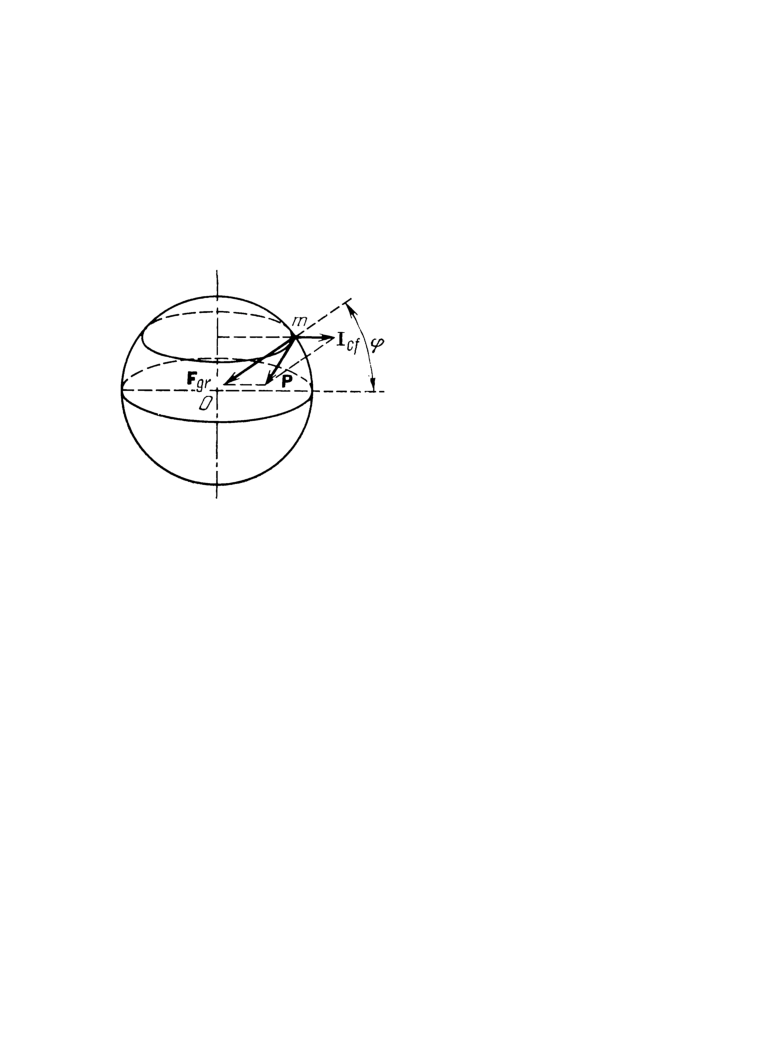
\includegraphics[width=0.8\textwidth]{figs/ch-07/fig-07-02.pdf}
%\input{figs/ch-03/fig-03-01}
%  \vspace{-13pt}
\sidecaption{The Coriolis force in a non-inertial frame of reference.\zhcap{非惯性参考系中的科里奥利力。}
\label{fig-07-02}}
\end{marginfigure}

\subsection{}\label{7.3.2} The \emph{gravity force of a body} is the force P, applied to the body and equal to the vector sum of the force $\vb{F}_{g\!r}$ of gravitational attraction of the earth for the body \ssect{6.1.3} and the centrifugal inertial force $\vb{I}_{c\!f}$ due to the diurnal rotation of the earth (\figr{fig-07-02}):
\zhpar{\emph{物体的重力}是作用于物体上的力 $\vb{P}$，它等于地球对物体的引力 $\vb{F}_{g\!r}$（\ssect{6.1.3}）与地球周日自转引起的惯性离心力 $\vb{I}_{c\!f}$ 的矢量和（见\figr{fig-07-02}）：}
\begin{equation*}%
\vb{P} = \vb{F}_{g\!r} + \vb{I}_{c\!f}.
\end{equation*}
i.e.
\zhpar{即}
\begin{equation*}%
\vb{P} = - G \frac{mM_{\Earth}}{r^{3}}\vb{r} - m \qty[\pmb{\Omega}[\pmb{\Omega}\vb{r}]].
\end{equation*}
Here $m$ and $M_{\Earth}$ are the masses of the body and the earth, $\vb{r}$ is the radius vector drawn from the centre of the earth to the place where the body is located, $\pmb{\Omega}$ is the angular velocity of diurnal rotation of the earth, and $G$ is the gravitational constant \ssect{6.1.1}.
\zhpar{式中 $m$ 与 $M_{\Earth}$ 分别为物体与地球的质量，$\vb{r}$ 为从地心指向物体所在位置的位矢，$\pmb{\Omega}$ 为地球周日自转的角速度，$G$ 为引力常量（\ssect{6.1.1}）。}

The gravity force causes an unsupported or unfastened body to fall to the earth. It equals the force with which the body presses against a horizontal support (or pulls on a vertical suspension) due to the gravitation attraction of the earth. It can be measured in the terrestrial frame of reference by means of a spring dynamometer. The point of application of the gravity force acting on a body, i.e. the point of appli­cation of the resultant of all the gravity forces acting on all the particles of the body is called the \emph{centre of gravity of the body}. It coincides with its centre of mass \ssect{2.3.3}.
\zhpar{重力使不受支承或未被固定的物体落向地球。它等于由于地球引力作用，物体对水平支承面施加的压力（或对竖直悬线施加的拉力）。它可以在地球固连参考系中用弹簧测力计测量。作用于物体上的重力的作用点，即作用于物体所有质点上的重力合力的作用点，称为\emph{物体的重心}。重心与物体的质心重合（\ssect{2.3.3}）。}

\subsection{}\label{7.3.3} The gravity force of a body is independent of its velocity of relative motion. It is proportional to the mass $m$ of the body and can be presented in the form
\zhpar{物体的重力与其相对运动速度无关。它与物体的质量 $m$ 成正比，可以写成如下形式：}
\begin{equation*}%
\vb{P} = m\vb{g},
\end{equation*}
where $\vb{g}$ is the \emph{acceleration due to gravity}, or \emph{free fall acceleration} (see \ssect{7.3.5}). At a given place on earth, vector $\vb{g}$ is the same for all bodies and changes for other places.
\zhpar{式中 $\vb{g}$ 称为\emph{重力加速度}，或称\emph{自由落体加速度}（见\ssect{7.3.5}）。在地球上某一地点，矢量 $\vb{g}$ 对所有物体都相同，在不同地点则不同。}

The gravity force of a body coincides with the gravitational attraction of the earth for the body only at the earth's North and South poles because there the centrifugal inertial force $\vb{I}_{c\!f} = 0$. The greatest difference between the gravity force and the gravitational attraction is observed at the equator, where the force $\vb{I}_{c\!f}$ reaches its maximum value and is opposite in direction to $\vb{F}_{g\!r}$. Even at the equator, however, the gravity force and the force of gravitational attraction differ by only 0.35 per cent. At all points of the earth's surface, except the equator and the poles, forces $\vb{P}$ and $\vb{F}_{g\!r}$ fail to coincide in direc­tion as well (\figr{fig-07-02}), but the maximum angle between them does not exceed 6 minutes of arc. The gravity force decreases with the altitude. Near the earth's surface this decrease is approximately 0.034 per cent per kilometre above the surface. 
\zhpar{物体的重力仅在地球南北两极处与地球对物体的引力重合，因为该处的惯性离心力 $\vb{I}_{c\!f} = 0$。重力与引力的差别在赤道处最大，此处惯性离心力 $\vb{I}_{c\!f}$ 达到最大值，且方向与 $\vb{F}_{g\!r}$ 相反。然而，即使在赤道处，重力与引力之差也仅为 0.35\%。在地球表面除赤道与两极以外的所有点上，$\vb{P}$ 与 $\vb{F}_{g\!r}$ 的方向也不一致（见\figr{fig-07-02}），但两者之间的最大夹角不超过 6 角分。重力随高度的增加而减小，在地球表面附近，每升高 1 千米，重力约减小 0.034\%。}

\subsection{}\label{7.3.4} The acceleration $\vb{g}$ near the earth's surface varies from \SI{9.78}{\meter\per\second\squared} at the equator to \SI{9.83}{\meter\per\second\squared} at the North and South poles. This is due, in the first place, to the dependence of the centrifugal inertial force on the geographical latitude of the location and, in the second, to the non-spherical shape of the earth, which is slightly flattened at the poles of its axis of rotation, having the shape of an ellipsoid of rotation, or sphe­roid (the polar and equatorial radii of the earth are $R_{p} = \SI{6357}{\kilo\meter}$ and $R_{e} = \SI{6378}{\kilo\meter}$). The \emph{standard value of free fall acceleration}, accepted in establishing a system of units and for barometric computation, is \SI{9.80665}{\meter\per\second\squared}.
\zhpar{地球表面附近的重力加速度 $\vb{g}$，在赤道处为 \SI{9.78}{\meter\per\second\squared}，在南北两极处为 \SI{9.83}{\meter\per\second\squared}。造成这一差异的原因，首先是惯性离心力随地理纬度而变化；其次是地球并非正球形，而是沿自转轴方向略扁，呈旋转椭球体（即扁球体）的形状（地球的极半径与赤道半径分别为 $R_{p} = \SI{6357}{\kilo\meter}$ 与 $R_{e} = \SI{6378}{\kilo\meter}$）。在建立单位制以及进行气压计算时所采用的\emph{自由落体加速度标准值}为 \SI{9.80665}{\meter\per\second\squared}。}

\subsection{}\label{7.3.5} The \emph{free fall of a body} is its motion due to the action of the gravitational held alone.
\zhpar{\emph{自由下落}是指物体仅在引力场作用下的运动。}

The free fall acceleration of a body falling to the earth, mea­ sured in a non-inertial frame of reference rotating together with the earth, can he found by the motion equation \ssect{7.3.1} by putting $\vb{F} = 0, \,\, \vb{F}_{g\!r} + \vb{I}_{c\!f} = m\vb{g}$ and $I_{C} = 2m \qty[\vb{v}_{r}\pmb{\Omega}]$. Then
\zhpar{落向地球的物体的自由落体加速度，若在随地球一起转动的非惯性参考系中测量，可由运动方程（\ssect{7.3.1}）求得。取 $\vb{F} = 0, \,\, \vb{F}_{g\!r} + \vb{I}_{c\!f} = m\vb{g}$，并取 $I_{C} = 2m \qty[\vb{v}_{r}\pmb{\Omega}]$，则有：}
\begin{equation*}%
\vb{a}_{r}= \vb{g} + 2\qty[\vb{v}_{r}\pmb{\Omega}].
\end{equation*}
If $\vb{v}_{r} = 0, \,\, \vb{a}_{r} = \vb{g}$.
\zhpar{若 $\vb{v}_{r} = 0$，则 $\vb{a}_{r} = \vb{g}$。}

Consequently, vector $\vb{g}$ is equal to the free fall acceleration of the body, measured with respect to the terrestrial frame of reference at the instant when the relative velocity of the body equals zero. For this reason, vector $\vb{g}$ is called the \emph{free fall acceleration}.
\zhpar{因此，矢量 $\vb{g}$ 等于物体在相对速度为零的瞬间，相对于地球固连参考系测得的自由落体加速度。正因如此，矢量 $\vb{g}$ 被称为\emph{自由落体加速度}。}

If the relative velocity of a freely falling body $\vb{v}_{r}=0$, its acceleration with respect to the earth is not $\vb{g}: \vb{g} = \vb{a}_{r}+ 2\qty[\vb{v}_{r}\pmb{\Omega}]$. At velocities $v_{r} < \SI{680}{\meter\per\second}$, however, the values of $\vb{g}$ and $\vb{a}_{r}$ differ by less than one per cent. It can therefore be assumed in many cases that with respect to an observer on the earth free fall of a body is caused only by the gravity force acting on and imparting the acceleration g to the body. In a similar manner the action of the Coriolis inertial force on a freely falling body can be treated as a comparatively small perturbation. Thus, for instance, a freely falling body is deviated by the Coriolis force to the east of the direction assumed by a plumb line, i.e. from the direction of the vector $\vb{P} = m\vb{g}$. This devia­tion for a body falling freely without any initial velocity from the height $h$ is equal, at the latitude $\varphi$, to
\zhpar{若自由下落物体的相对速度 $\vb{v}_{r}=0$，则其相对于地球的加速度并不等于 $\vb{g}$：$\vb{g} = \vb{a}_{r}+ 2\qty[\vb{v}_{r}\pmb{\Omega}]$。然而，当速度 $v_{r} < \SI{680}{\meter\per\second}$ 时，$\vb{g}$ 与 $\vb{a}_{r}$ 的数值相差小于 1\%。因此，在许多情况下，对于地球上的观察者而言，可以认为物体的自由下落仅由重力引起，重力使物体获得加速度 $\vb{g}$。同样，科里奥利惯性力对自由下落物体的作用，可视为较小的微扰。例如，自由下落的物体会受到科里奥利力的作用，从铅垂线所指的方向（即矢量 $\vb{P} = m\vb{g}$ 的方向）向东偏离。对于从高度 $h$ 处无初速自由下落的物体，其偏离量在纬度 $\varphi$ 处由下式给出：}
\begin{equation*}%
s = \frac{2}{3} \Omega h \sqrt{\dfrac{2h}{g}} \cos \varphi.
\end{equation*}
If, for example, $h = \SI{160}{\meter}$ and $\varphi = \ang{45},\,\, s = \SI{1.55}{\centi\meter}$. 
\zhpar{例如，若 $h = \SI{160}{\meter}$，$\varphi = \ang{45}$，则 $s = \SI{1.55}{\centi\meter}$。}

\subsection{}\label{7.3.6} The \emph{weight of a body} is the force $\vb{Q}$ with which it acts, due to the earth's gravity, on a support or suspension that prevents it from falling freely. It is assumed that the body and its support (or suspension) are fixed with respect to the frame of reference in which the weight is determined. The force $-\vb{Q}$ is exerted by the support or suspension on the body. It follows from the fundamental equation of dynamics of rela­tive motion \ssect{7.2.2}, where $\vb{a}_{r} =\vb{a}_{C} = 0$ and $\vb{F} = \vb{F}_{g\!r} - \vb{Q}$, that
\zhpar{\emph{物体的重量}是指：由于地球引力作用，物体对阻止其自由下落的支承物或悬挂物所施加的力 $\vb{Q}$。假定物体及其支承物（或悬挂物）相对于确定重量所用的参考系是静止的。支承物（或悬挂物）对物体施加的反作用力为 $-\vb{Q}$。由相对运动动力学基本方程（\ssect{7.2.2}，其中 $\vb{a}_{r} =\vb{a}_{C} = 0$，$\vb{F} = \vb{F}_{g\!r} - \vb{Q}$）可得：}
\begin{equation*}%
\vb{Q} = \vb{F}_{g\!r} + \vb{I}_{t},
\end{equation*}
where $\vb{F}_{g\!r}$ is the force of gravitational attraction of the earth for the body, and $\vb{I}_{t}$ is the inertial force of transportation due to the non-inertial nature of the frame of reference. 
\zhpar{式中 $\vb{F}_{g\!r}$ 为地球对物体的引力，$\vb{I}_{t}$ 为由参考系的非惯性性质引起的牵连惯性力。}

\noindent\hlblue{Example 1.} The weight of a body in a frame of reference fixed to the earth is equal to the gravity force of the body \ssect{7.3.2}:
\zhpar{\hlblue{例 1.} 在固连于地球的参考系中，物体的重量等于该物体的重力（\ssect{7.3.2}），如下式所示：}
\begin{equation*}%
\vb{Q} = \vb{F}_{g\!r} + \vb{I}_{c\!f} = \vb{P}.
\end{equation*}
\hlblue{Example 2.} The weight of a body in a frame of reference at­tached to a lift (elevator) which travels with translational motion with respect to the earth with the acceleration $\vb{a}_{0}$:
\zhpar{\hlblue{例 2.} 在固连于电梯（升降机）的参考系中，电梯相对于地球以加速度 $\vb{a}_{0}$ 作平动，此时物体的重量如下式所示：}
\begin{equation*}%
\vb{Q} = \vb{P} - m \vb{a}_{0}.
\end{equation*}
If the lift falls freely, $\vb{a}_{0}= \vb{g}$, the free fall acceleration, and the weight of the body in the lift is $\vb{Q} = 0$, i.e. the body is in the state of weightlessness.
\zhpar{若电梯自由下落，则 $\vb{a}_{0}= \vb{g}$，即自由落体加速度，此时电梯中物体的重量 $\vb{Q} = 0$，即物体处于失重状态。}

\subsection{}\label{7.3.7} \emph{Weightlessness}, or zero gravity, is the state of a mechan­ical system in which the external gravitational field acting on the system does not cause any pressure of the parts against one another or their deformation. Such a state occurs in a me­chanical system complying with the following three conditions: 
\zhpar{\emph{失重}，或称零重力，是指机械系统所处的这样一种状态：作用于该系统的外部引力场不会引起各部分之间的压力，也不会引起其变形。满足下列三个条件的机械系统即处于此种状态：}
\begin{enumerate}[label=(\alph*)]
\item no other external forces, except those of the gravitational field, act on the system; 
\zhpar{除引力场的作用外，没有其他外力作用于系统；}
\item the size of the system is such that within its limits the external gravitational field can be regarded
as being uniform; and 
\zhpar{系统的尺寸足够小，使得在其范围内外部引力场可以视为均匀场；并且}
\item the system is in translational motion. 
\zhpar{系统处于平动状态。}
\end{enumerate}
The state of weightlessness is characteristic, for instance, of bodies in a spaceship because, during the main part of its path in a gravitational field, it is in free flight, i.e. coasting with the engines turned off.
\zhpar{失重状态例如出现在宇宙飞船中的物体上，因为宇宙飞船在引力场中的大部分飞行过程中处于自由飞行状态，即关闭发动机后的惯性滑行。}

\section{Principle of Equivalence}
\label{sec-7.4}
\zhtitle{等效原理}

\subsection{}\label{7.4.1} The inertial forces acting on bodies in a non-inertial frame of reference are proportional to the masses of the bodies and, other conditions being equal, impart the same relative accelerations \ssect{7.1.3} to them. In other words, all bodies free of external action travel in an ``inertial force field'', i.e. with respect to a non-inertial frame of reference, in absolutely the same way, provided that the initial conditions of their motion are also the same. A similar behaviour is observed for bodies travelling with respect to an inertial frame of reference and
\zhpar{作用于非惯性参考系中物体的惯性力与物体的质量成正比，并且在其他条件相同的情况下，会使物体获得相同的相对加速度（\ssect{7.1.3}）。换言之，在“惯性力场”中，所有不受外作用的物体，只要初始条件相同，相对于非惯性参考系的运动方式就完全相同。对于相对惯性参考系运动、并受引力场作用的物体，也观察到类似的行为：}

subject to the action of the forces of a gravitational field. At each point in the field these forces, like the inertial forces, are proportional to the masses of the bodies and impart the same free fall acceleration to them. This acceleration is equal to the field intensity \ssect{6.2.1} at the point being considered.
In a non-inertial frame of reference, for example, fixed to a lift (elevator) travelling with uniform acceleration vertically upward at the acceleration of transportation $\vb{a}_{0}= \textrm{const}$, all free bodies fall in the absence of a gravitational field with the same relative acceleration $\vb{a}_{r} = -\vb{a}_{0}$. Free bodies behave in exactly the same way in the same lift when it travels at uni­form velocity in a uniform gravitational field of the intensity $\vb{g}_{f} = -\vb{a}_{0}$. Thus, on the basis of experiments conducted on the free fall of bodies within a tightly closed lift, it is impossible to establish whether the lift is travelling at uniform velocity in a gravitational field of the intensity $\vb{g}_{f} = \vb{a}_{r}$ (in partic­ular, the lift may also be at rest in this held) or whether it is travelling with constant acceleration of transportation $\vb{a}_{t} = -\vb{a}_{r}$ in the absence of a gravitational field.
\zhpar{在引力场的每一点上，这些力与惯性力一样，与物体质量成正比，并使物体获得相同的自由落体加速度，该加速度等于所考虑点处的场强（\ssect{6.2.1}）。例如，在固连于以恒定牵连加速度 $\vb{a}_{0}= \textrm{const}$ 竖直向上匀加速运动的电梯上的非惯性参考系中，在不存在引力场的情况下，所有自由物体都以相同的相对加速度 $\vb{a}_{r} = -\vb{a}_{0}$ 下落。同一电梯以匀速运动、处于场强为 $\vb{g}_{f} = -\vb{a}_{0}$ 的均匀引力场中时，自由物体的运动完全相同。因此，仅凭在封闭电梯内所做的自由落体实验，无法确定：电梯是以匀速运动并处于场强为 $\vb{g}_{f} = \vb{a}_{r}$ 的引力场中（特别地，电梯也可以静止于该场中），还是在无引力场的情况下以恒定牵连加速度 $\vb{a}_{t} = -\vb{a}_{r}$ 运动。}

\subsection{}\label{7.4.2} The \emph{local equivalence principle} states that the gravitational field in a limited region of space is equivalent to an ``inertial force held'' in a properly chosen non-inertial frame of reference. The region of space should be small enough so that the gravitational held in it can be assumed to be uniform.
\zhpar{\emph{局部等效原理}指出：有限区域内的引力场，等效于在适当选取的非惯性参考系中的“惯性力场”。该区域应足够小，使其中的引力场可以视为均匀场。}

The equivalence principle is not to be understood as a state­ment of the identity of inertial forces and Newton's gravita­tional forces that act between bodies. As a matter of fact, the intensity of a true gravitational held, set up by bodies, decreases as the bodies recede farther and farther away, and approaches zero at infinity. Gravitational fields ``equivalent'' to iner­tial forces do not comply with this condition. For example, the intensity of a gravitational held, ``equivalent'' to the centri­fugal inertial forces in a rotating frame of reference increases without limit at points farther and farther away from the axis of rotation. The intensity of a held ``equivalent'' to the inertial forces of transportation in a frame of reference having transla­tional motion is the same at all points of the held.
\zhpar{不应将等效原理理解为惯性力与物体之间的牛顿引力相同。事实上，真实引力场的场强随产生场的物体相互远离而减小，并在无穷远处趋于零。而与惯性力“等效”的引力场并不满足这一条件。例如，在旋转参考系中，与惯性离心力“等效”的引力场，其场强在远离转轴的点上无限增大。与平动参考系中牵连惯性力“等效”的引力场，其场强在场的所有点上都相同。}

\subsection{}\label{7.4.3} A true gravitational held, in contrast to one ``equivalent'' to inertial forces, exists in both non-inertial and inertial frames of reference. No possible choice of a non-inertial frame of ref­erence can completely eliminate a true gravitational held, i.e. compensate for it throughout space by means of a ``field of inertial forces''. This follows in any case, even if only from the different behaviour of ``fields of inertial forces'' and true gravitational fields at infinity. A true gravitational field can be eliminated only locally, i.e. for a small region of space within whose limits the field can he assumed uniform, and for a short time interval during which the field can be assumed constant. The non-inertial frame of reference corresponding to this operation should travel with an acceleration of transpor­tation equal to the free fall acceleration of bodies in the region of the true gravitational field being considered. Thus, in a space ship in free flight in a gravitational field, the gravitational forces of attraction are compensated for by the inertial forces of transportation and do not lead to the relative motion of bodies in the ship.
\zhpar{与“等效于惯性力”的引力场不同，真正的引力场既存在于非惯性参考系中，也存在于惯性参考系中。任何非惯性参考系的选取，都不能完全消除真正的引力场，即无法借助“惯性力场”在整个空间中对其加以补偿。至少由于“惯性力场”与真正引力场在无穷远处的行为不同，就足以得出这一结论。真正的引力场只能在局部被消除，即在一个足够小的区域（该区域内的场可视为均匀场）内、并在一个足够短的时间间隔内（该场可视为恒定）加以消除。与这一操作相应的非惯性参考系，应以等于所考虑真正引力场区域内物体自由落体加速度的牵连加速度运动。因此，在自由飞行于引力场中的宇宙飞船中，引力被牵连惯性力所补偿，从而不会引起飞船内物体的相对运动。}